\chapter{State of the art}
\label{chapter2}
\thispagestyle{empty}

\begin{quotation}
{\footnotesize
\noindent{\emph{``Rem tene, verba sequentur''}\\
(Know the subject, the words will follow)
}
\begin{flushright}
Marcius Porcius Cato Censorius
\end{flushright}
}
\end{quotation}
\vspace{0.5cm}

%\noindent Nella seconda sezione si riporta lo stato dell'arte del settore, un inquadramento dell'area di ricerca orientato a portare il lettore all'interno della problematica affrontata. Bisogna dimostrare di conoscere le cose fatte fino ad ora in questo campo e il perch\'e si sia reso necessario lo svolgimento di questo lavoro. Questa sezione deve essere grondante di citazioni bibliografiche \cite{Adaptative}.

\section{Background}

\indent \textit{Breast cancer classification} divides breast cancer into categories according to different schemes\footnote{\url{http://www.breastpathology.info/}}, each serving a different purpose.
The purpose of classification is to select the best treatment\cite{Genestie2011}.\\
Within the last decade, histological grading has become widely accepted as a powerful indicator of prognosis in breast cancer. 
The grading depends on the microscopic similarity of breast cancer cells to normal breast tissue, and classifies the cancer as well differentiated (low grade),
moderately differentiated (intermediate grade), and poorly differentiated (high grade), reflecting progressively less normal appearing cells that have a worsening prognosis.
Although grading is fundamentally based on how biopsied, cultured cells behave, in practice the grading of a given cancer is derived by assessing the cellular appearance of the tumor.\\
The \Gls{NGS} (also called Elston-Ellis) is a modification \cite{breastCancerGrading01} of the \Gls{BR}\cite{BRgrading01, BRgenestie}. \Gls{NGS}
is judged more reproducible and is the recommended grading method \cite{NGSrecommended}.


\Gls{NGS} grades breast carcinomas by adding up scores for:\\
\vbox{%
\begin{itemize}
\item tubule formation,
\item nuclear pleomorphism,
\item mitotic count
\end{itemize}}
each of which is given 1 to 3 points. The scores for each of these three criteria and then added together to give an overall final score and corresponding grade as follows \cite{damjanov2007cancer}:\\

\vbox{%
\begin{itemize}
 \item[3-5] \textbf{Grade 1 tumor} (well-differentiated). Best prognosis.
 \item[6-7] \textbf{Grade 2 tumor} (moderately-differentiated). Medium prognosis.
 \item[8-9] \textbf{Grade 3 tumor} (poorly-differentiated). Worst prognosis.
\end{itemize}}

Lower grade tumors, with a more favorable prognosis, can be treated less aggressively, and have a better survival rate.\\

Mitotic activity (see \ref{appendixA} for some details) is one of the strongest prognosticators for invasive breast carcinoma. It is expressed as the number of mitotic figures per tissue area.
Early detection plays an important role in reducing cancer mortality. The current procedure for breast cancer grading is manually performed by pathologists,
for both nuclear pleomorphism \cite{dunne2001scoring} and mitotic count.
Breast tissue samples of patients are taken and examined under microscopes. Pathologists grade the tissue samples based on the deviation of the cell structures
from normal tissues. A pathologist may have to examine a great amount of slides \cite{histopat01}. This process can be time consuming and subjective (see \ref{ch3:humans}).\\
In the following subsection we give a short overview of the mitosis count procedure\cite{amida13}.

\subsection{Tissue preparation}

After tumor excision is performed, the excised material is sent for analysis in a pathology lab.
The tissue preparation process starts with making smaller cuts of the material that are then fixed
in formalin and (after processing) embedded in paraffin.\\
Using a high precision cutting instrument (microtome), thin sections are cut from the
paraffin block, which are then put on glass slides. The final stage of the tissue
preparation process is the staining of the sections with stains that highlight specific
structures of the tissue so they are better visible under a microscope.
The standard staining protocol uses the \Gls{HE} stains.
The hematoxylin dyes the nuclei a dark purple color and the eosin
dyes other structures (cytoplasm, stroma, etc.) a pink color.

\subsection{Digital Pathology}

Recent years have brought the trend of digitization of histological slides. Digital slide
scanners \ref{ch2:fig1}, in combination with digital slide viewers, aim to provide the experience of
viewing a digital slide on a computer monitor in a manner analogous to viewing it under
a microscope, but with all the added benefits of the digital format (ease of annotation,
image analysis, collaborative viewing etc.).
The output of the digital slide scanners are multi-layered images, stored in a format that
enables fast zooming and panning. Depending on the area of the tissue that is present on
the slide and the magnification and resolution at which the slide is scanned, the lowest
layer of the digital slide can be up to several tens of thousands of pixels in width or
height.
Currently, digital slides are mainly used for research, education and remote consultation
purposes. Their use for routine diagnosis and prognosis is not yet common \cite{histopatholImaging01}.
Availability of automatic image analysis algorithms that can aid pathologists in their work can be a major incentive for
acceptance of digital slides in the routine pathology lab workflow.

\begin{figure}[!hbf]
 \begin{center}
  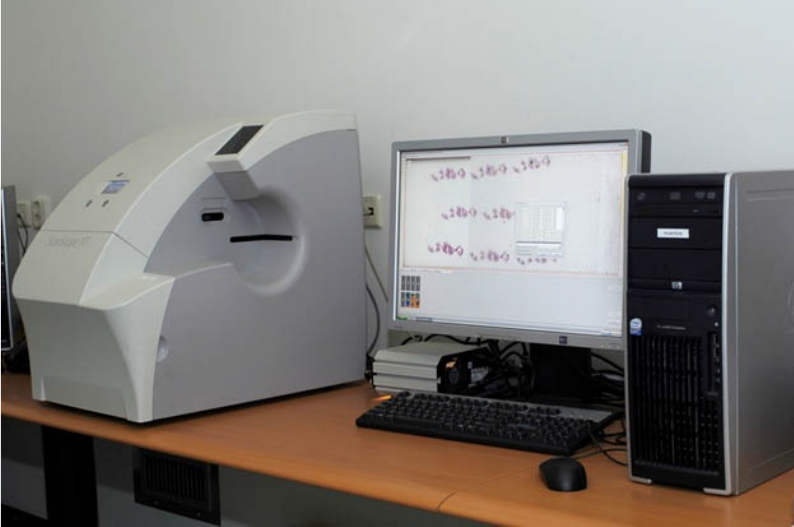
\includegraphics[width=0.6\textwidth]{./images/aperio.png}
  \caption{Aperio ScanScope XT scanner}
  \label{ch2:fig1}
 \end{center}
\end{figure}

\subsection{Mitosis Counting}
Mitotic activity is one of the strongest prognosticators for invasive breast carcinoma and it
is expressed as the number of mitotic figures per tissue area. As part of the \Gls{BR} grading system, mitotic activity is
routinely assessed in pathology labs across the world. In addition, the mitotic activity
can be used as a prognosticator independently of the \Gls{BR} grading system.
Typically, the pathologist receives a panel of slides for each case that is to be graded. He
or she then proceeds to select one slide where the histological grading will be
performed. The mitosis counting is performed in 8-10 consecutive microscope \Gls{HPF} \cite{breastCancerMitosisPCA_ICA}. 
A HPF has a size of $512 \times 512 \mu m^{2}$ (i.e. an area of 0.262 $mm^{2}$ ), which is the equivalent of a microscope field diameter of $0.58mm$.
The standard guidelines are to select an area that encompasses the most invasive
part of the tumor, at the periphery and with highest cellularity. Depending on the
number of figures counted, a mitotic activity score is assigned. Cases with 7 or fewer
mitotic figures present are assigned score 1 (best prognosis). Cases with more than 12
mitotic figures are assigned score 3 (worst prognosis). The intermediate cases are
assigned score 2.

\subsection{Challenges in Mitosis Detection}
Because of the aberrant chromosomal makeup of many tumors (aneusomy, polysomy,
translocations, amplifications, deletions), the appearance of mitotic figures in the
images can significantly differ from the textbook examples of a splitting nucleus\cite{mitosisDetectBreastCancer01}. In
addition, imperfections of the tissue preparation process result in tissue appearance
variability, which can present a challenge also for an automated mitosis detection system.\\
Most commonly, mitotic figures are exhibited as hyperchromatic objects. In addition,
they have absence of a clear nuclear membrane, \textquotedblleft hairy\textquotedblright protrusions around the edges
and basophilia instead of eosinophilia of the surrounding cytoplasm. However, these are
more guidelines than hard rules, and the bulk of the training of pathologists is done by
looking as specific examples of mitotic figures.
One of the main challenges in spotting mitotic figures is that other objects such as
apoptotic nuclei can have similar appearance, making it
difficult even for trained experts to make a distinction \cite{mitosisDetectionLearningBased}. Lymphocytes, compressed
nuclei, \textquotedblleft junk\textquotedblright particles and other artifact form the tissue preparation process, can also
have hyperchromatic appearance.
The images in Figures \ref{ch2:fig2}, \ref{ch2:fig3} and \ref{ch2:fig3b} try to give an idea of the difficulty of the task.

\begin{figure}[!hbt]
  \centering
    \subfigure[]{
      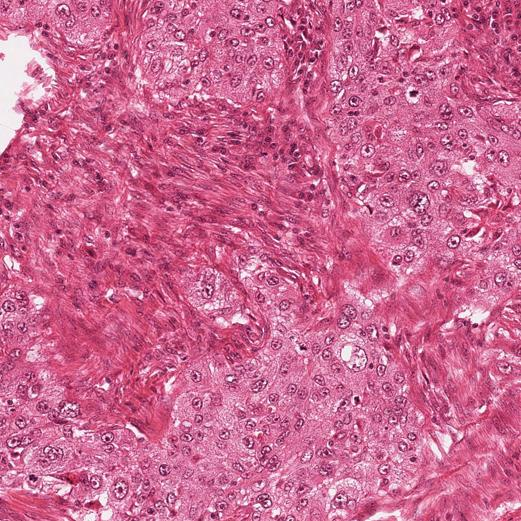
\includegraphics[width=0.44\textwidth]{./images/A00_06th.jpg}
      \label{ch2:fig2:a}
    }
    \hspace{2mm}
    \subfigure[]{
      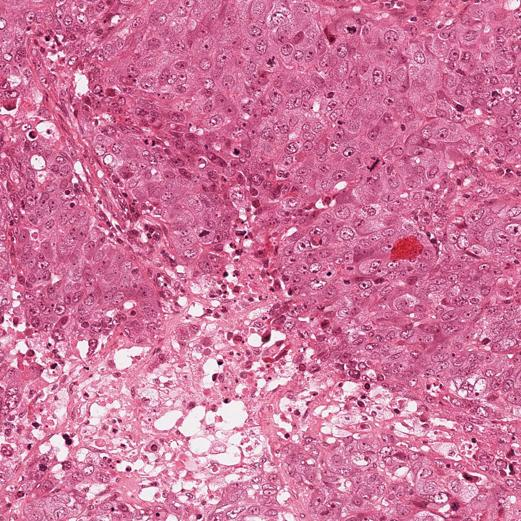
\includegraphics[width=0.44\textwidth]{./images/A01_05th.jpg}
      \label{ch2:fig2:b}
    }\\
    \vspace{2mm}
    \subfigure[]{
      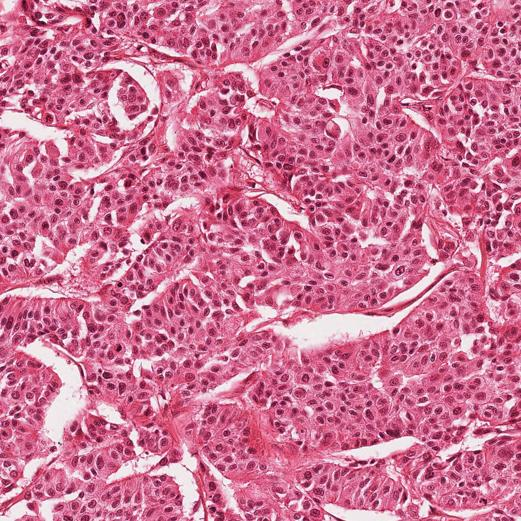
\includegraphics[width=0.44\textwidth]{./images/A02_02th.jpg}
      \label{ch2:fig2:c}
    }
    \hspace{2mm}
    \subfigure[]{
      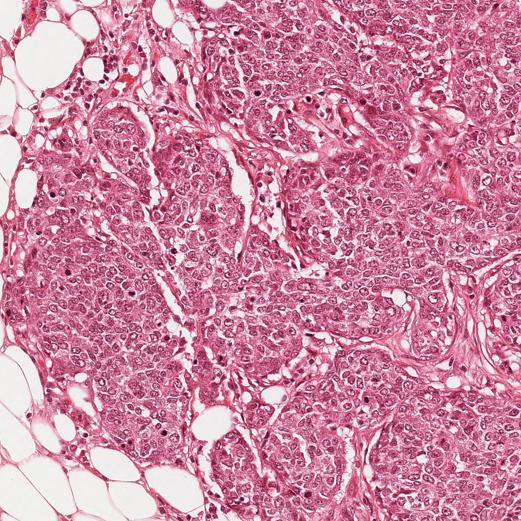
\includegraphics[width=0.44\textwidth]{./images/A03_02th.jpg}
      \label{ch2:fig2:d}
    }
    \caption{Examples of digital histological images}
    \label{ch2:fig2}
\end{figure}

\vspace{0.5cm}

\section{Mitosis Detection and Computer Vision}


The task of automatic mitosis detection involves topics in varius fields of research, in particular

\begin{itemize}
 \item Image Analysis
 \item Machine Learning
\end{itemize}

We consider a framework in which, in the whole image, some candidates are detected and the classified as mitosis or non-mitosis.\\
In this chapter we give an overview of the main aspects concerning \textit{image analysis} and in the following one (\ref{ch2:ML}) we analyze the \textit{machine learning} elements.




\subsection{Overview of Medical Imaging}

Over the past decade, dramatic increases in computational power and improvement in image analysis algorithms have
allowed the development of powerful computer-assisted analytical approaches to radiological and histo-pathological data\cite{HistopatImaging01Review}.
Digitized tissue histopathology has now become ame-nable to the application of computerized image analysis and machine learning techniques.
Analogous to the role of \Gls{CAD} algorithms in medical imaging to complement the opinion of a radiologist, \Gls{CAD} algorithms have begun to be developed for
disease detection, diagnosis, and prognosis prediction to complement the opinion of the pathologist\cite{sertel2009computer}.

\subsection{Software Tools}

The imaging modalities rely heavily on computational approaches. In fact, in many cases the computational technology is just as important as the optics,
not just for the digital capture that all systems now use but in many cases also for visualizing and properly interpreting the data.
The article in 	\cite{BioImagingSW05} reviews each computational step that biologists encounter when dealing with digital images and the overall status of available software for bioimage informatics.
It is worth highlighting the existence of open-source software tools like \textit{Fiji} \cite{BioImagingSW03} and \textit{ImageJ} \cite{BioImagingSW02}, which supply some basic features
for \textit{object detection} and \textit{feature extraction}\cite{featuresReviewBioinformatics}.

\vspace{0.5cm}


\subsection{Features}

The concept of feature is used to denote a piece of information which is relevant for solving a computational task\cite{featExtractionAndImageProcessingBook}.
A feature is defined as an \textquotedblleft{interesting}\textquotedblright part of an image, and features are used as a starting point for many \Gls{CV} algorithms.
They can be the result of a general \textit{neighborhood operation}\cite{jahne2000computer} applied to the image, or specific structures in the image itself.
Types of image features include:
\begin{itemize}
 \item Edges
 \item Corners
 \item Blobs or \Glspl{ROI}
 \item Ridges or elongated objects (i.e. blood vessels in medical images)
\end{itemize}

Other examples of features are related to motion in image sequences, to shapes defined in terms
of curves or boundaries between different image regions, or to properties of such a region\cite{MVG_Hartley2004}.

The feature concept is very general and the choice of features in a particular \Gls{CV} system may be highly dependent on the specific problem to be considered.\\


\subsection{Feature Detectors}

Many algorithms have been developed to detect specific features, and a complete overview of them is beyond
the scope of this work. Some of the most famous ones, like \textit{Canny edge detector}\cite{canny},
\textit{Harris edge and corner detector}, or SUSAN \cite{detectSusan} are available in most widely used
commercial and open-source Computer Vision software packages (i.e. {\scshape Matlab}
Image Processing Toolbox\footnote{\url{http://www.mathworks.com/products/image/index.html}} or OpenCV\footnote{\url{http://opencv.org/}} ).\\

Features are sometimes extracted over several scalings. One of these methods is \textit{Scale-invariant feature transform};
in this algorithm, various scales of the image are analyzed to extract features\cite{LoweScale} (the underlying theory can be found in \cite{feature01ScaleSpace}).\\


\subsection{Image Segmentation}
\label{ch2:IS}
Segmentation is the process of partitioning a digital image into multiple segments (sets of pixels) in order to simplify
or change the representation of an image into something that is more meaningful and easier to analyze\cite{breastCancer02}.
Image segmentation is typically used to locate objects and boundaries (i.e. features) in images. 
Such a process assigns a label to every pixel in an image so that pixels with the same label share certain visual characteristics\cite{mitosisDetectionLearningBased}.


\subsection{Texture Algorithms}

An image texture is a set of metrics designed to quantify the perceived texture of an image.
Image texture gives information about the spatial arrangement of color or intensities in an image or in selected region of it\cite{ CV_Forsyth}.
Image textures are used in \textit{segmentation}(see \ref{ch2:IS}), or \textit{classification} of images (see \ref{ch2:ML}).
To address the issue of texture analysis, the so called \textquotedblleft{}statistical approach\textquotedblright  is more widely used as it is easier to compute.
This approach sees an image texture as a quantitative measure of the arrangement of intensities in a region.

\subsubsection{Co-occurrence Matrix}

Co-occurrence matrix captures numerical features of a texture using spatial relations of similar gray tones.
Numerical features computed from the co-occurrence matrix can be used to represent, compare, and classify textures\cite{textureGLCMexample, textureGLCM_wood}.
The following are a subset of standard features derivable from a normalized co-occurrence matrix, as described in \cite{haralick1973textural}:

\begin{eqnarray}
\textrm{Contrast} & = & \sum_{n=0}^{N_g-1} n^{2} \left\{ \sum_{i=1}^{N_g} \sum_{j=1}^{N_g} p[i,j] \right\}, \ \textrm{where} |i-j| = n \\
\textrm{Correlation} & = & \frac{ \sum_{i=1}^{N_g} \sum_{j=1}^{N_g} (i,j) \cdot p[i,j] - \mu_x \mu_y }{\sigma_x \sigma_y} \\
\textrm{Entropy} & = & - \sum_{i} \sum_{j} p[i,j] \cdot \log(p[i,j])
\end{eqnarray}

Where:
\begin{itemize}
 \item $N_g$ is the number of gray levels in the quantized image,
 \item $p[i,j]$ is the $(i,j)th$ entry in a normalized gray-tone spatial dependence matrix,
 \item $\mu_x,\sigma_x,\mu_y,\sigma_y$ are the mean and the standard deviation of respectively $p_x = \sum_{j=1}^{N_g}p(i,j)$ and  $p_y = \sum_{i=1}^{N_g}p(i,j)$.
\end{itemize}

Various algorithms use texture feature like \Gls{GLCM} \cite{texture03}, \Gls{GLRM} \cite{texture02} or \Gls{GLEM} for image classification,
also in medical \cite{texture04} and biological imaging \cite{textGLCMbiol}.


\subsubsection{Local Binary Patterns}

\Gls{LBP} is another type of feature used for classification in Computer Vision. \Gls{LBP} is a simple yet very efficient texture operator
which labels the pixels of an image by thresholding the neighborhood of each pixel with the value of the center pixel and considers the result as a binary number.
The distance and the number of neighbors can be selected, as shown in Figure \ref{ch2:fig4}\cite{LBP01}.
The notation $(P,R)$ is used for pixel neighborhoods which means \textit{P} sampling points on a circle of radius of \textit{R}.

\begin{figure}[!htb]
  \centering
    \subfigure[(8,1)]{
      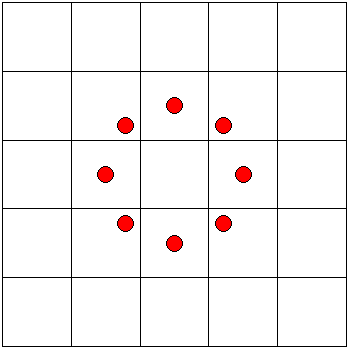
\includegraphics[width=0.25\textwidth]{./images/lbp1_c.png}
      \label{ch2:fig4:a}
    }
    \hspace{1mm}
    \subfigure[(8,2)]{
      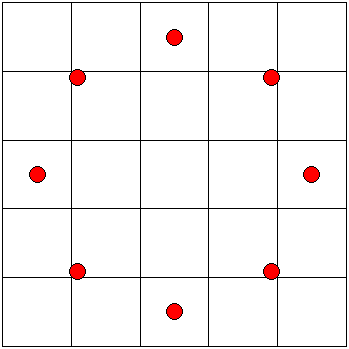
\includegraphics[width=0.25\textwidth]{./images/lbp2_c.png}
      \label{ch2:fig4:b}
    }
    \hspace{1mm}
    \subfigure[(16,3)]{
      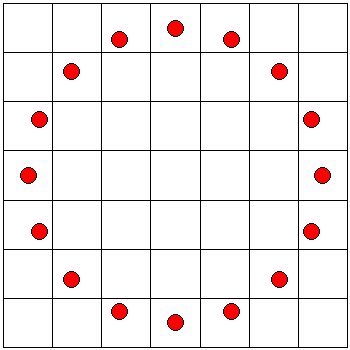
\includegraphics[width=0.25\textwidth]{./images/lbp3_c.png}
      \label{ch2:fig4:c}
    }    
    \caption{Examples LBP neighbors and distances}
    \label{ch2:fig4}
\end{figure}

The computation of the \Gls{LBP} code of a pixel of coordinates $(x_c,y_c)$ is given by:

\begin{equation}
 LBP_{P,R} = \sum_{p=0}^{P-1} s(g_p - g_c) \cdot 2^{p} \quad \textrm{where} \ s(x) = 
    \left\{
	\begin{array}{ll} 1, & \textrm{if} \ x \geq 0\\
			  0, & \textrm{otherwise}
	\end{array}
    \right.
\end{equation}

This operator used jointly with a simple local contrast measure provided very good performance in unsupervised texture segmentation.
Another extension to the original operator is the definition of so called uniform patterns, which can be used to reduce the length of the feature
vector and implement a simple rotation-invariant descriptor. This extension was inspired by the fact that some binary patterns occur more commonly
in texture images than others. A \Gls{LBP} is called uniform if the binary pattern contains at most two bitwise transitions from 0 to 1
or vice versa when the bit pattern is traversed circularly.\\
. In the computation of the \Gls{LBP} labels, uniform patterns are used so that there is a separate label for each uniform pattern and all
the non-uniform patterns are labeled with a single label.
For example, when using $(8,R)$ neighborhood, there are a total of 256 patterns, 58 of which are uniform, which yields in 59 different labels. 

The uniform and rotation invariant \Gls{LBP}  can be further enhanced by combining it with a \Gls{VAR} operator, with the same parameters $(P,R)$,
that characterizes the contrast of local image texture\cite{LBP02}.
Both operators are also computationally attractive, as they can be realized with a few operations in a small neighborhood and a lookup table.
The \Gls{VAR} operator is described by the following relations:

\begin{equation}
 VAR_{(P,R)} = \frac{1}{P} \sum_{p=0}^{P-1}(g_p - \mu)^{2} \quad \textrm{where} \ \mu = \sum_{p=0}^{P-1}g_p^2
\end{equation}

\Gls{LBP}$(P,R)$ and \Gls{VAR}$(P,R)$ are complementary and a feature set made by the combination of the two is expected to be a very
powerful rotation invariant measure of local image texture. It is also possible to use joint feature sets composed by operators with different neighborhood.

\subsubsection{Wavelets}

The \Gls{WT} is having greater importance medicine and biology.
The main uses of the \Gls{WT} concern the analysis of one-dimensional physiological signals obtained by electrocardiography (ECG)
and electroencephalography (EEG), including evoked response potentials\cite{wavelets}.
A survey of recent wavelet developments in medical imaging can be found in \cite{waveletsBiomed}.
These include biomedical image processing algorithms (e.g., noise reduction, image enhancement, and detection) and
image reconstruction and acquisition schemes (tomography, and \Gls{MRI}).


\subsection{Object detection and recognition}

Object detection is a Computer Vision technology that deals with detecting instances of semantic objects of a certain class (such as humans, traffic signs, mitotic cells) in digital images
Humans recognize a multitude of objects in images with little effort, despite the fact that the image of the objects may be in different orientation,
or in different size/scale. Objects can even be recognized when they are partially obstructed from view.
This task is still a challenge for \Gls{CV} systems and represents the connection between Image Analysis topics and Machine Learning.
Viola and Jones proposed a well known object detection framework \cite{objDetect04ViolaJones, objDetect05ViolaJonesRapid}, which involves the sums
of image pixels within rectangular areas, using the so-called Haar-like features, a name that resembles the Haar wavelet adopted in \cite{objDetect03framework}.
The technique generates a large amount of features and uses the boosting algorithm \textit{AdaBoost} to reduce the over-complete set, by selecting the best features and training classifiers that use them.
The evaluation of the classifiers generated in the learning phase can be quick, but generally not enough to be run in real-time. For this reason, the classifiers are arranged in a cascade in order of complexity,
where each susequent classifier is trained only on those selected samples which pass through the preceding classifiers.
If at any stage in the cascade a classifier rejects a sample, no further processing is performed.
The cascade therefore has the form of a degenerate tree.


\vspace{0.5cm}

\begin{figure}[!hpbt]
 \centering
  \subfigure[source image]{
    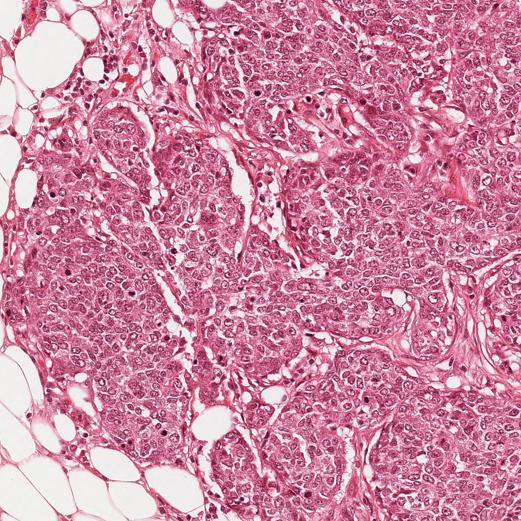
\includegraphics[width=0.64\textwidth]{./images/A03_02th.jpg}
    \label{ch2:fig3:a}
   }\\
  \subfigure[mitoses]{
    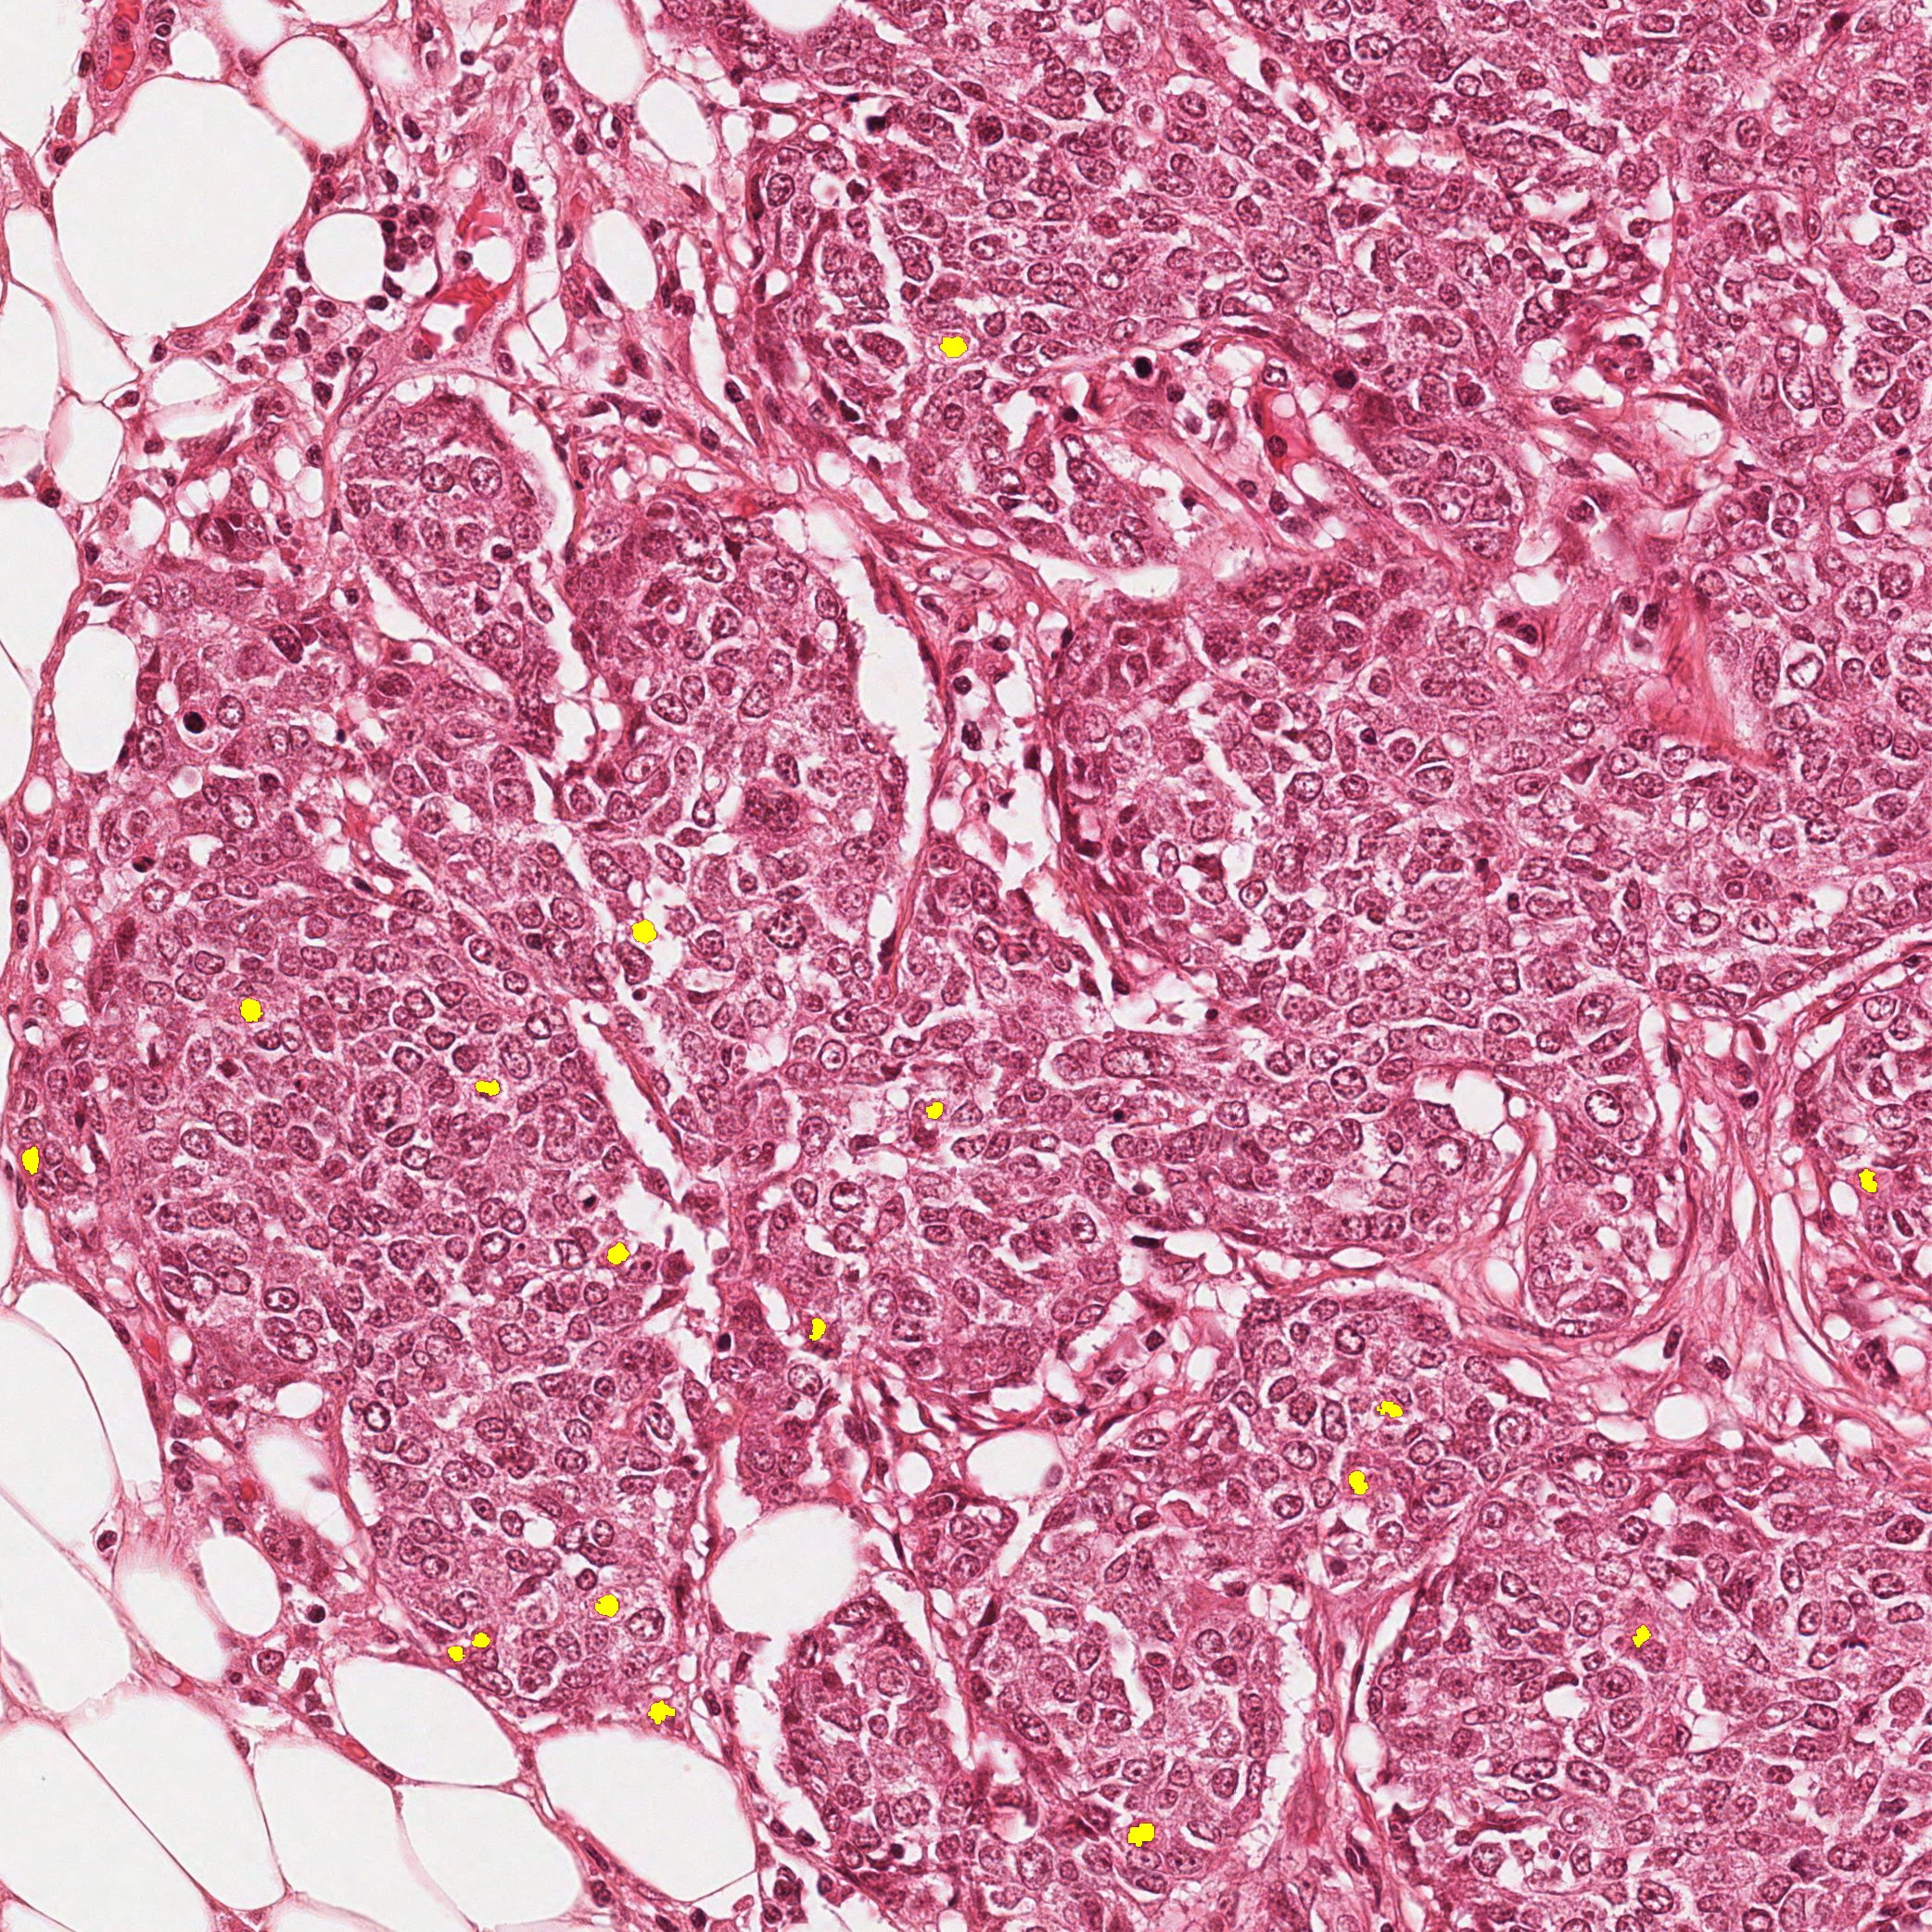
\includegraphics[width=0.64\textwidth]{./images/A03_02.jpg}
    \label{ch2:fig3:b}
  }
  \caption[Example of image with highlighted mitoses]{Example of image with highlighted mitoses (yellow) }
  \label{ch2:fig3}
\end{figure}


\begin{figure}[!hpbt]
 \centering
  \subfigure[source image (zoom)]{
    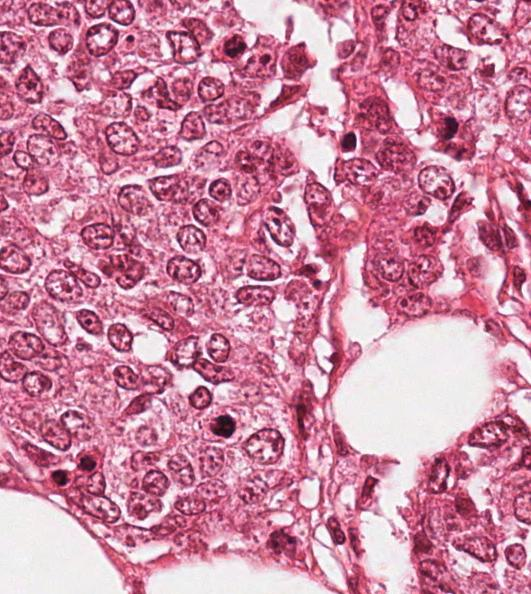
\includegraphics[width=0.64\textwidth]{./images/A03_02th_z.jpg}
    \label{ch2:fig3b:a}
   }\\
  \subfigure[mitoses (zoom)]{
    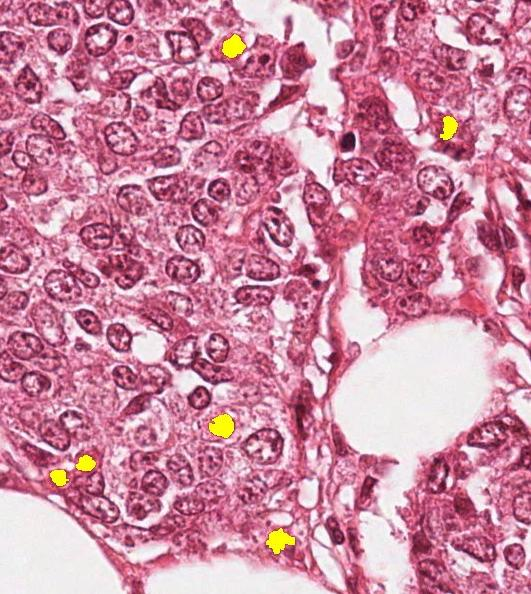
\includegraphics[width=0.64\textwidth]{./images/A03_02_z.jpg}
    \label{ch2:fig3b:b}
  }
  \caption[Detail of Figure \ref{ch2:fig3}]{Example of image with highlighted mitoses (yellow) detail of Figure \ref{ch2:fig3} }
  \label{ch2:fig3b}
\end{figure}

\clearpage

\section{Machine Learning}
\label{ch2:ML}

\Gls{ML}, a branch of \Gls{AI}, deals with the ability to define and to build systems that can learn from data.
The core of \Gls{ML} deals with the representation of data and their generalization. Representation deals with the way the system describes the data.
Generalization deals with the ability of the system to perform on unseen data samples.
In Machine Learning, the observations are often known as \textit{instances},
the explanatory variables are termed \textit{features} (grouped into a \textit{feature vector}), and the possible categories to be predicted are \textit{classes}. 


\Gls{ML} algorithms can be divided into different types:
\begin{itemize} 
 \item [-] \textbf{Supervised Learning} generates a function that maps inputs to desired outputs usually called \textit{labels},
	because they are often provided by human experts classifying the training examples.
 \item [-] \textbf{Unsupervised learning} models a set of inputs. It can also be referred to as \textit{data mining} and knowledge discovery. Here, labels are not known during training.
 \item [-] \textbf{Semi-supervised learning} combines both labeled and unlabeled examples to generate an appropriate function or classifier. 
 \item [-] \textbf{Reinforcement learning} learns how to act given an observation of the world. Every action has some impact in the environment, and the environment provides feedback in the form of rewards that guides the learning algorithm.
\end{itemize}

There exists a great variety of \Gls{ML} algorithms, and a detailed review is beyond the scope of this work\footnote{A list of \Gls{ML} algorithms can be found in
\url{http://en.wikipedia.org/wiki/List_of_machine_learning_algorithms}}.\\
We focous, in our analysis, on \textit{Pattern Recognition} and in particular on \textit{Supervised Learning} methods.

\subsection{Pattern Recognition}
\label{ch2:pr}
\Gls{PR} is the assignment of a label to a given input value \cite{bishop2006pattern, theodoridis2008pattern}. In its most general form, \Gls{PR} involves:

\begin{itemize}
 \item \textbf{Classification} is the problem of identifying to which of a set of categories a new observation belongs, on the basis
 of a training set of data containing instances whose category membership is known,
 \item \textbf{Regression} is a technique for estimating the relationships among variables, assigning a real-valued output to each input,
 \item \textbf{Sequence labeling} refers to the assignment of a categorical label to each member of a sequence of observed values,
 in particular by making choices which depend on the one made for nearby elements (e.g. speech tagging)
 \item \textbf{Parsing} is the process of analyzing a string of symbols according to the rules of a formal grammar.
\end{itemize}

\subsection{Classification}

Among the different types of learning methods and pattern recognition techniques we focus our attention on \textit{classification} which, in general \Gls{ML} 
terminology, is an instance of \textit{supervised learning}.\\
The formal definition of a supervised classification problem can be stated as follows: an unknown function $g$ maps the input instances $x \in X$ to the output labels $y \in Y$:

\begin{equation}
 \label{ch2:eq1}
 g: X \rightarrow Y
\end{equation}

Equation \ref{ch2:eq1} represents the \textit{ground truth}.\\
The \textit{training set}
\begin{equation}
 T = { (x_1,y_1), \ldots ,(x_n,y_n) }
\end{equation}

is assumed to represent the mapping of $g$ in an accurate way. The classifier then tries to build a function $h: X \rightarrow Y$ that approximates as closely as possible the correct mapping. The measure of the performance
(see \ref{ch3:perf} for details) is generally done on a separate set of data ( the \textit{test set}) whose labels are known but whose data are not used during the learning phase\cite{liu2006pattern}.

A common subclass of classification is \textit{probabilistic classification}. Algorithms of this type involve statistical tools to define the best class for a given instance\cite{ML_gaussian}.
Probabilistic algorithms output a probability that the instance is a member of each of the possible classes. The best class is normally then selected as the one with the highest probability.
Classification can be also divided into two separate problems - \textit{binary classification} and \textit{multi-class classification}.
In binary classification, only two classes are involved, whereas multi-class classification considers the problem of assigning an object to one of several classes.
Since many classification methods have been developed specifically for binary classification, multi-class classification often requires the combined use of multiple binary classifiers.

\subsection{Binary Classification}

Binary classification is the task of classifying the members of a given set of objects into two groups on the basis of whether they have some property or not\cite{scholkopf2002learning}.
Medical testing is a typical binary classification task (i.e. to determine if a patient has certain disease or not ).
In traditional statistical hypothesis testing, the tester starts with a null hypothesis and an alternative hypothesis,
performs an experiment, and then decides whether to reject the null hypothesis in favor of the alternative.
Hypothesis testing is therefore a binary classification of the hypothesis under study \cite{mitchML}.
A \textit{positive} result is one which rejects the null hypothesis.
Rejecting the null hypothesis when it is actually true - a \Gls{FP} - is a \textbf{type I error};
on the other hand, when the null hypothesis is false results in a \Gls{TP}.
A \textit{negative} result is one which does not reject the null hypothesis.
Accepting the null hypothesis when it is actually false - a \Gls{FN} - is a \textbf{type II error};
on the other hand, when the null hypothesis is true results in a \Gls{TN}.
How the number of \Gls{TP}, \Gls{FP}, \Gls{TN} and \Gls{FN} can be used to assess the performances of a classification algorithm is treated in Section \ref{ch3:perf}.


\subsection{Binary Classifiers}

An algorithm that implements a classification, is defined a \textbf{classifier}.
The term also refers to the mathematical function, implemented by a classification algorithm, that maps input data to a category (i.e. \textit{class}).
A great amount of algorithms has been developed for classification purposes, in particular for \Gls{CV} tasks \cite{classificationSurvey}.
Some methods suitable for learning binary classifiers include\cite{dataMiningBook}:

\begin{itemize}
 \item Naive Bayes classifiers
 \item Bayesian networks \ \cite{bayesClassifiersCellSegmentation}
 \item Decision trees \ \cite{randTree01}
 \item \Glspl{RF} \ \cite{randForests01}
 \item \Glspl{SVM} \ \cite{SVM01}
 \item Hidden Markov models
 \item \Glspl{NN} \ \cite{russell2010artificial}
\end{itemize}


In our work we focused on two types of classifiers: \textit{Support Vector Machines} and \textit{Random Forests}
which are widely used in \Gls{CV} classification problems ( e.g. \cite{mitosisDetectionLearningBased} and \cite{randForests04}).

\subsection{Software Tools}

Classification tasks can be accomplished by a large amount of software tools. Here we mention the ones that we consider to be the most relevant ones.\\
\textit{Weka} \cite{dataMining_Weka, dataMining_Weka_upd} is a \textbf{FLOSS} general purpose data mining software tool developed by the Waikato University
\footnote{\url{http://www.cs.waikato.ac.nz/ml/weka/}} which allows to implement a great variety of classifiers \cite{dataMiningBook}. It also has an interface
with \textbf{R} \footnote{\url{http://cran.r-project.org/}} \cite{hornik2009open}.\\
{\scshape Matlab} can perform classification task by means of some of its toolboxes (i.e. Bioinformatics \footnote{\url{http://www.mathworks.com/products/bioinfo/} }
and Statistics \footnote{\url{http://www.mathworks.com/products/statistics/} } ).


\vspace{0.5cm}

